\documentclass[12pt,a4paper]{article}
\usepackage{fancyhdr}
\usepackage{fontspec}
\usepackage{amsmath}
\usepackage{amssymb}
\usepackage{bm}
\usepackage{tikz}
\setmainfont{Microsoft YaHei}
\pagestyle{fancy}

\begin{document}

\fancyfoot[C]{by chinasjtu@msn.com }

\newcommand{\nl}{\newline}

\newcommand{\ntinf}{\lim\limits_{n \to \infty}}
\newcommand{\xtinf}{\lim\limits_{x \to \infty}}

\newcommand{\Atinf}{\lim\limits_{A \to \infty}}
\newcommand{\Rtinf}{\lim\limits_{R \to \infty}}

\newcommand{\ntx}[1]{\lim\limits_{n \to #1}}
\newcommand{\xtx}[1]{\lim\limits_{x \to #1}}
\newcommand{\ttx}[1]{\lim\limits_{t \to #1}} 
\newcommand{\ktx}[1]{\lim\limits_{k \to #1}} 
\newcommand{\dxtx}[1]{\lim\limits_{\Delta x \to #1}}

\newcommand{\jfab}{\int_{a}^{b}}
\newcommand{\jf}[2]{\int_{#1}^{#2}}

\newcommand{\nsum}[2]{\sum\limits_{n=#1}^{#2}}
\newcommand{\isum}[2]{\sum\limits_{i=#1}^{#2}}
\newcommand{\ksum}[2]{\sum\limits_{k=#1}^{#2}}

\newcommand{\nsuminf} {\nsum{1}{\infty}}
\newcommand{\ksuminf} {\ksum{1}{\infty}}
\newcommand{\isuminf} {\isum{1}{\infty}}




\begin{center} 选优试题  \end{center}

1995

$1.设E为满足下列条件的非负非空数集$

$(i)supE=\mu<1;(ii)\forall x,y \in E,x<y有\frac{x}{y}\in E$

$证明必有\mu \in E$

$\nl$

$2.设0<x_1<x_2<...<x_n<\pi,证明:\prod\limits_{i=1}^N \frac{sinx_i}{x_i} \le (\frac{sinx}{x})^n$

$其中x=\frac{1}{n}\isum{1}{n}x_i$

$\nl$

$3.(1)设f(x)在[a,b]上无界,证明\exists \epsilon \in [a,b],使得\forall \delta >0,f(x)在\cup(\epsilon,\delta)\cap [a,b]上无界$

$(2)试构造[0,1]上的函数f(x),使得它在(0,1)内任一点的任意小领域内都无界$

$\nl$

$4.设f(x)在[0,1]上可导,f'(x) \in R[0,1],又\int_{0}^{1}f(x)dx=0,证明$

$\int_{0}^{1}f^2(x)dx \le \int_{0}^{1}[f'(x)]^2dx$

$\nl$

$5.设f(x)在[-1,1]上无穷次可导,f(\frac{1}{n})=\frac{n^2}{1+n^2},n \in \bold N,求f^{(k)}(0),k \in \bold N$

$\nl$

$6.设f(x)\in R[a,b],f(x)>0,x\in[a,b],证明\jfab f(x)dx>0(区间套)$

$\nl$

$7.设f(x)在[0,+\infty)上一致连续,证明\forall \alpha>0,有\xtinf \frac{f(x)}{x^{1+\alpha}}=0$

$\nl$

1996

$1.设数列\{x_n\}由方程x_n^3+2x_n+\frac{1}{n}=0,n\in \bold N的实根定义,证明数列\{nx_n\}收敛,并求其极限值$

$\nl$

$2.(1)试构造函数f(x),使其在[0,1]上处处不连续,但可取到最大值,最小值及一切中间值$

$(2)试构造函数f(x),使其在[0,1]上一致连续,但不满足Lipshity条件$

$\nl$

$3.设f''(x)\in C[0,1],且f(0)=0,f''(x)>0,\forall x \in [0,1].证明唯一存在点\epsilon \in (0,1)使得$

$(1+\epsilon)f'(\epsilon)-f(\epsilon)=f(1)$

$\nl$

$4.设f(x) \in C[0,1],g(x)在[0,1]上单调递增,若对\forall [a,b] \subset [0,1],都有|\jfab f(x)dx|^2 \le [g(b)-g(a)](b-a)$

$证明:(\jf{0}{1}|f(x)|dx)^2 \le g(1)-g(0)$

$\nl$

$5.设数列a_0,a_1,a_2,...,a_n...满足$

$a_n=\ksum{1}{\infty}tg^2a_{n+k},n=0,1,...$

$若级数\nsum{0}{\infty}a_n 收敛,证明a_n \equiv 0,n=0,1,...$

$\nl$

$6.设函数列\{f_n(x)\}在[a,b]上一致收敛,f_n(x)\in C[a,b],n \in \bold N,记h(x)=sup_n\{f_n(x)\}$

$证明h(x) \in C[a,b]$

$\nl$

$7.设f(x)在[0,1]上全体有理点处连续,证明f(x)至少在[0,1]的某个无理点处连续$

$又若f(x)在[0,1]上全体无理点处连续,能否证明f(x)至少在[0,1]的某个有理点处连续$

$\nl$

$1.设a>0,取x_1>a^{\frac{1}{p}}(p \in N),x_{n+1}=\frac{p-1}{p}x_n+\frac{a}{p}x_n^{1-p},n=1,2,...$

$证明数列\{x_n\}收敛,并求其极限值$

$\nl$

$2.设f(x)\in C[0,1],f(0)=f(1),证明对\forall n \in N,相应有x_n \in [0,1],使得$

$f(x_n)=f(x_n+\frac{1}{n})$

$\nl$

$3.设f''(x) \in C[0,1],f(0)=f(1),又\exists M>0,使|f''(x)|\le M,x \in [0,1]$

$证明|f'(x)|\le \frac{M}{2},x \in [0,1]$

$\nl$

$4.图中抛物线为y=x-x^2,直线y=c及y轴与抛物线所围两块阴影部分面积分别为A_1,A_2,$

$试在下列情况下分别确定C之值$

$(1)使得A_1=A_2;(2)使得A_1+A_2取最小值$

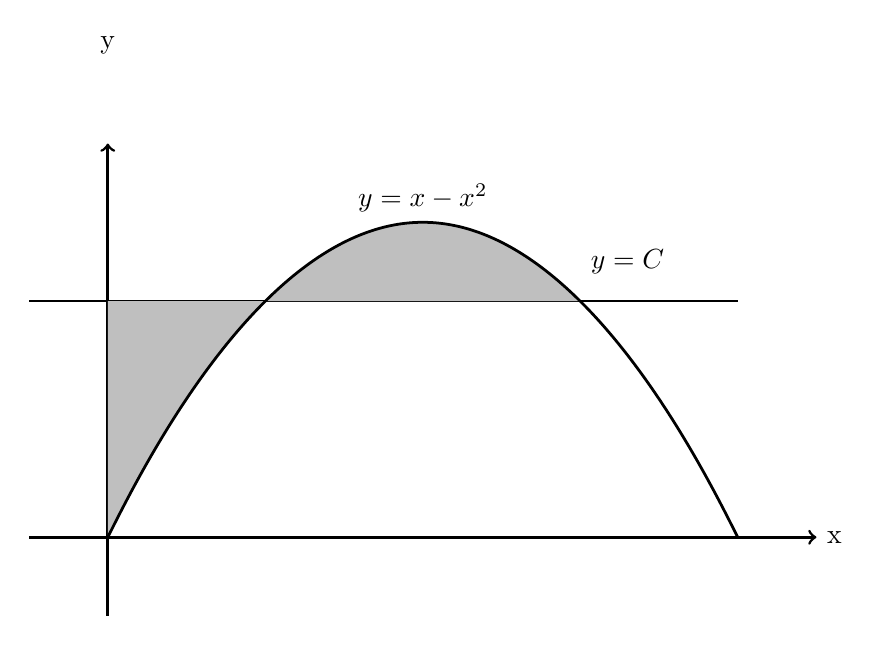
\begin{tikzpicture}[domain=1:5,line width=1pt]
\draw[->] (-1,0) -- (9,0);
\draw[->] (0,-1) -- (0,5);

\draw (-1,3) -- (8,3);

\node [right] at (9,0) {x};
\node [above] at (0,6) {y};
\node [above] at (4,4) {$y=x-x^2$};
\node [right] at (6,3.5) {$y=C$};

\path[fill=gray!50]  (0,3)--(6,3)--(6,3) parabola bend (4,4) (0,0);

\draw (0,0) parabola bend (4,4) (8,0);
        
\end{tikzpicture}

$6.设f(x)在[a,+\infty)上可导,f'(x)为可积函数,当x \to +\infty 时f(x)单调递减趋于0$

$又\jf{a}{+\infty}f(x)dx 收敛,证明\jf{a}{+\infty}xf'(x)dx 收敛且$

$\jf{a}{+\infty}xf'(x)dx=-\jf{a}{+\infty}f(x)dx-af(a)$

$\nl$

$1997$

$1.试构造数列\{x_n\},使其对\forall a \in [0,1],\exists \{x_{n_k}\} \subset \{x_n\},满足$

$\ktx{\infty}x_{n_k}=a$

$\nl$

$4.设f(x) \in C[a,b],在(a,b)内处处存在右导数f_+'(x),且f(a)=f(b)=0,证明$

$证明:\exists c \in (a,b),使得f_+'(c) \le 0$

$\nl$

$5.设C(\alpha)是(1+x)^{\alpha}在x=0处Taylor公式中x^{1197}的系数,试求$

$I=-\jf{0}{1}C(-1-y)\isum{1}{1997}\frac{1}{y+i}dy$

$\nl$

$6.设f'(x) \in C[a,+\infty),且A>0,使得$

$|f'(x)|\le A|f(x)|,\forall x \in [a,+\infty)$

$又f(a)=0,证明f(x) \equiv 0,x \in [a,+\infty)$

$\nl$

$7.设f'(x) \in C[a,b],且\jfab f(x)dx=0,证明$

$\jfab f^2(x)dx \le \frac{(b-a)^2}{2}\jfab [f'(x)]^2dx$

$\nl$

$8.设数列\{a_n\}单调递增,且a_n>0(n \in N),\lambda > 0,证明级数$

$\nsum{1}{\infty}\frac{a_{n+1}-a_n}{a_{n+1}a_n^{\lambda}}收敛$

$\nl$

$9.(1)求极限\xtinf \nsum{1}{\infty}\frac{x^2}{n(2n+1)x^2+n+x}$

$(2)求和\isum{1}{\infty}\jsum{1}{\infty}\frac{(-1)^{i+j}}{i+j}$

1998

$\nl$

$1.设\{x_n\}为非负递增数列,且对\forall m,n \in N,有x_{mn}\ge mx_n,若$

$sup_n \{\frac{x_n}{n}\}=c常数$

$证明\ntinf \frac{x_n}{n}=c$

$\nl$

$2.设f(x)在(a,b)内可导,\xtx{a^+}f(x)=+\infty,试问是否必有\xtx{a^+}|f'(x)|=+\infty$

$是否必有\overline{ \xtx{a^+} }|f'(x)|=+\infty$

$\nl$

$3.设正项级数\nsum{1}{\infty}a_n,其部分和为S_n-\ksum{1}{n}a_k ,证明$

$(1)\nsum{1}{\infty}\frac{a_n}{S_n}也发散$

$(2)\nsum{1}{\infty}\frac{a_n}{S_n^ \lambda }收敛(\lambda >0)$

$\nl$

$4.设f(x)=(\alpha - \frac{1}{\alpha}-x)(4-3x^2),证明f(x)恰好有一个极大值与一个极小值$

$若把这两个值之差记为\Delta (\alpha),试求\Delta (\alpha) 关于\alpha 的最小值$

$\nl$

$5.设f(x)在[a,b]上可导,f'(x) \in R[a,b],记$

$x_k=a+k\frac{b-a}{n}(k=0,1,...n),A(n)=\frac{b-a}{n}\ksum{1}{n}f(x_k)-\jfab f(x)dx$

$试求\ntinf nA(n)之值$

$\nl$

$6.引进‘稠密’概念如下:设E为R上数集,若对\forall x \in [a,b],存在E中点列\{x_n\},$

$使得\ntinf x_n=x,称E在[a,b]中稠密$

$现设f(x)为[a,b]上非负可积函数,且\jfab f(x)dx=0,记$

$E={x|f(x)=0,x\in [a,b]}$

$证明E在[a,b]中稠密$

\newpage


\begin{center} 第一讲 极限与连续  \end{center}


$例:设\{x_n\}由方程x_n^3+2x_n+\frac{1}{n}=0,n \in N的实根确定,证明\{nx_n\}收敛,并求出极限值$

$证明:显然x_n<0,f'(x=(x^3+2x)'>0.反证法:设x_{n_0+1}<x_{n_0}$

$则有x_{n_0+1}^3+2x_{n_0+1}<x_{n_0}^3+2x_{n_0}与方程矛盾,x_n递增有上界\ntinf x_n=0$

$因为nx_n=-\frac{1}{x_n^2+2},故\ntinf nx_n=-\frac{1}{2}$

$\nl$

$例:设正项级数\nsuminf a_n收敛,\{y_n\}定义为y_1=1,2y_{n+1}=y_n+\sqrt{y_n^2+a_n}n\in N$

$证明\{y_n\}收敛$

$证明:单调性易证,由4y_{n+1}^2-4y_{n+1}y_n=a_n \to y_{n+1}-y_n=\frac{a_n}{4y_{n+1}} \to y_{n+1}-y_n < a_n$

$两边同取部分和,故y_{n+1}<1+S_{(a_n)}$

$\nl$

$例:设f(x)在[a,b]上严格递增,对\{x_n\} \subset [a,b]有\ntinf f(x_n)=f(a),证明:\ntinf x_n=a$

$反证思路:若\ntinf x_n \ne a,则必有sup \ntinf x_n=c>a,从而有子列\ntinf x_{n_k}=c$

$于是\exists k_0:\forall k>k_0,有x_{n_k}>\frac{a+c}{2}>a,故f(n_k)>f(\frac{a+c}{2}),即有f(x_{n_k})-f(a)$

$>f(\frac{a+c}{2})-f(a),取\epsilon_0=f(\frac{a+c}{2})-f(a)>0,\exists N:f(x_n)-f(a)<f(\frac{a+c}{2})-f(a)$

$\nl$

$例:引进“稠密概念”设E \subset R为数集,若对每一个x \in D,在点x的任意邻域$

$内至少含有E中的一个点,称E在D上稠密。设\{x_n\}为有界数列,且满足x_n-x_{n+1}<\alpha_n$

$其中\alpha_n \to 0,证明\{x_n\}在其上下极限之间稠密$

$分析:若\overline {lim} x_n = \underline {lim}x_n,无须证明。设M=\overline {lim} x_n > \underline {lim}x_n = m ,任取l>2,充分大(l \in N)$

$记\frac{M-m}{l} \triangleq \delta >0,用分点-\infty,m+\delta,m+2\delta,...M-2\delta,M-\delta,+\infty$

$将\bold{R}分为l个区间,取充分大N,使得\forall n>N时,有|\alpha_n|<\delta,再取$

$n_2>n_1>N:x_{n_1} \in (M-\delta,+\infty)x_{n_2} \in (-\infty,m+\delta),则可证在区间$

$[m+\delta,m+2\delta]....[M-2\delta,M-\delta]上每一个中至少含有\{x_n\}中一点x_k$

$(n_1 < k < n_2),倘若不然,至少存在上述区间中某个记为(a,b)$

$b-a=\delta,中不含\{x_n\}中点,则由区间构造及x_k(n_1<k n_2)的各点取法$

$可知必有在某个k,x_k \ge b,x_{k+1}\le a,于是x_k-x_{k+1} \ge b-a$

$=\delta > |\alpha_n|\ge \alpha_n 与条件矛盾,因此每一个x \in [m,M]及\forall \epsilon >0$

$取l充分大,总可以使\frac{M-m}{l} \triangleq \delta < \epsilon,从而使U(x,\epsilon)中至少存在$

$\nl$

$例:设e^xf(x),e^{-f(x)}在(0,1)内单调递增,证明f(x)\in C[0,1]$

$只需证\xtx{x_0^-}f(x)=\xtx{x_0^+}f(x)=f(x_0),\forall x_0 \in (0,1)$

$当x>x_0时有e^xf(x) \ge e^{x_0}f(x_0)及e^{-f(x)}\ge e^{-f(x_0)}从而有$

$f(x_0)-f(x) \ge 0,即e^{x_0-x}f(x_0)\le f(x) \le f(x_0)故有$

$\xtx{x_0^+}f(x)=f(x_0)$

$\nl$

$例:f(x)\in C(a,b),f^2(x)在(a,b)一致连续。证明:f(x)在(a,b)内一致连续$

$要证\xtx{a+}f(x)\xtx{b-}f(x)存在,因为f^2(x)一致连续,故\xtx{a}f^2(x)=A$

$A=0时,\xtx{a+}f(x)=0,当A>0时,\xtx{a+}|f(x)|=\sqrt A,\exists \delta >0:|f(x)|>\frac{\sqrt A}{2}$

$\forall x \in [a,a+\delta),故f(x)不变号在[a,a+\delta)否则有零点,必有\xtx{a+}f(x)=\sqrt A$

$\nl$

$设f(x)在[0,+\infty)上一致连续,证明对\forall \alpha >0,有\xtinf \frac{f(x)}{x^{1+\alpha}}=0$

$分析:证\exists A,B>0,使得|f(x)|\le A|x|+B$

$\nl$

$例:设f(x)g(x)均为[1,+\infty)上非负一致连续,且xf(x)也一致连续$

$证明:(1)f(x),\frac{g(x)}{x}在[1,+\infty)上有界(2)f,g在(1,+\infty)啥一致连续$

$(1)记|g(1)|\triangleq  c,\epsilon = 1,\exists \delta>0: |g(1)-g(1+\frac{\delta}{2})|<1$

$|g(1+\frac{\delta}{2})-g(1+2\frac{\delta}{2})|<1$

$故|g(1+k\frac{\delta}{2})-g(1)|<k,\frac{g(1+k\frac{\delta}{2})}{1+k\frac{\delta}{2}}<\frac{c+k}{k\frac{\delta}{2}},从而\frac{g(x)}{x}有界$

$证(2):\forall \epsilon >0,\exists \delta>0,x|f(x)-f(y)| \le \epsilon,\forall x,y \in(1,+\infty)$

$由(1)\exists M>0,f(x) \le M,故\exists \delta >0(0<\delta<\frac{\epsilon}{2M},|x-y|<\delta)$

$使得当|x-y|<\delta,有x|f(x)-f(y)|\le|xf(x)-yf(y)|+f(y)|x-y|$

$<\frac{\epsilon}{2}+M\frac{\epsilon}{2M},再证f(x)g(x)一致连续,\exists \delta >0,使得当|x-y|<\delta$

$|g(x)-g(y)|<\frac{\epsilon}{2M},y|f(x)-f(y)|<\frac{\epsilon}{2M}$

$|f(x)g(x)-f(y)g(y)|<f(x)|g(x)-g(y)|+\frac{g(y)}{y}y|f(x)-f(y)|$

$<M_1\frac{\epsilon}{2M_1}+M_2\frac{\epsilon}{2M_2}$

$\nl$

$设f:R \to R 为连续映射。\exists a \in R与c>0,\forall n有|f^n(a)|\le c证明$

$f在R上有一个不动点x_0$

$反证法:设f(x)>x,\forall x \in R,令x_1=a,x_{n+1}=f(x_n)则\{x_n\}有界$

$x_{n+1}=f(x_n)>x_n,故可记\lim x_n=x_0,则x_0=f(x_0)$

$\nl$

$设I \subset R为闭区间,映射f:I \to I满足|f(x)-f(y)|<|x-y|$

$\forall x,y \in I,证明:f在I上有不动点$

$任取x \in I,令x_{n+1}=f(x_n)则\{x_n\} \subset I,则有|x_{n+1}-x_n|<|x_n-x_{n-1}|$

$故\{|x_{n+1}-x_n|\}单调递减有下界,记\ntinf |x_{n+1}-x_n|=a \ge 0$

$有界,由致密性定理,\exists \{x_{n_k}\} \subset \{x_n\}:\ntinf x_{n_k}=x_0,由题可推知f \in C(Z)$

$故有\ntinf x_{n_k+1}=\ntinf f(x_{n_k})=f(x_0) \triangleq x^*, \ntinf x_{n_k+2}=f(x^*)$

$|x_{n_k+2}-x_{n_k+1}|=|f(x_{n_k+1})-f(x_{n_k})|<|x_{n_k+1}-x_{n_k}|即有$

$|f(x^*)-f(x_0)|=|x^*-x_0|,由题设x^*=x,f(x_0)=x_0$

$\nl$

\begin{center} 一致收敛及其应用  \end{center}


$一、概念与定理小结$

$(1)f_n(x) \overset{\underset{\mathrm{D}}{}}{\rightrightarrows} f(x)(或S_n(x)\overset{\underset{\mathrm{D}}{}}{\rightrightarrows}  S(x))$

$1'按定义,\forall \epsilon >0,\exists N \in \bold{N}:\forall n>N,\forall x \in D:|f_n(x)-f(x)|<\epsilon$

$2' Cauchy准则,\forall \epsilon >0,\exists N \in \bold N:\forall n>N;\forall p \in \bold N,\forall x \in D,|f_{n+p}(x)-f_n(x)|<\epsilon$

$3'按确界极限,\ntinf sup_D|f_n(x)-f(x)|=0$

$4'点到极限,\ntinf |f_n(x_n)-f(x_n)|=0,\forall \{x_n\} \subset D(充要条件)反证法$

$\exists \epsilon_0,\forall N \in N,\exists n_0 >N及 \zeta_0 \in D:|f_{n_0}(\zeta_0)-f(\zeta_0)|\ge \epsilon_0$

$\nl$

$例:证明:\{x^ne^{-n^2x}\}在[0,+\infty)区间一致收敛,\{\frac{nx}{n^2+(n+1)x}\}在[0,+\infty)上不一致收敛,取x_n=n$

$求sup|f_n(x)=f(x)|时应详细说明极值,驻点旁增减性相异。$

$\nl$

$(2)判别法,①M-判别法,|n_n(x)| \le a_n,\sum a_n 收敛,\sum|n_n(x)|收敛$

$②Dirichlet Abel ③Dini ④Lzberniz法,设U_n(x) \rightrightarrows (D) 0, 0 \le U_{n+1}(x) \le U_n(x)$

$\forall n \in N(\forall x \in D),则交错级数\sum (-1)^nU_n(x)在D上一致收敛$

$\nl$

$(3)解析性 ①连续性②可积性③可微性$

$\nsuminf (\frac{nx}{1+n^2x^2}-\frac{(n-1)x}{1+(n-1)^2x^2}),x \in [0,1]部分和级数为S_n(x)=\frac{nx}{1+n^2x^2},x \in(0,1)$

$S(x)=0,取x_n=\frac{1}{n},但⒈ \ntinf \xtinf S_n(x)=\xtinf \ntinf S_n(x)=0$

$⒉0=\jf{0}{1}\lim S_n(x)dx=\ntinf \jf{0}{1}S_n(x)dx=0,⒊\sum(\frac{nx}{1+n^2x^2}-\frac{(n-1)x}{1+(n-1)^2x^2})在[0,1]$

$上不一致收敛,但0=\frac{d}{dx}\lim S_n(x)=\lim \frac{d}{dx}S_n(x)=0$

$①\forall \epsilon >0, \{f_n(x)\}在[a,b-\epsilon]上一致收敛,是否必有\{f_n(x)\}在[a,b)上一致收敛.反例:f(x)=x^n,[0,1]$

$②若\{f_n(x)\}在[a,b)内一致收敛,且\{f_n(b)\}收敛,是否必有\{f_n(x)\}在[a,b]上收敛,可证$

$③若\sum U_n(x)在(a,b)一致收敛,U_n(x) \in C[a,b],\forall n \in N,是否必有\sum U_n(x)在[a,b]上一致收敛,对$

$④若有D上处处不连续f_n(x) \forall n \in N,f_n(x) \rightrightarrows (D) f(x)是否必有f(x) \notin C(D),反例:f_n(x)=
\begin{cases}
\frac{1}{n},x \in Q \\
0,x \notin Q
\end{cases}
$

$⑤f_n(x) \in C[a,b],f_n(x) \rightrightarrows (D) f(x),故\{x_n\} \subset [a,b],\ntinf x_n=x,是否必有\ntinf f_n(x_n)=f(x),拆项证明$

$\nl$

$设U_n(x) \in C[a,b],\forall n \in N, \sum U_n(x)在[a,b)内一致收敛,证明$

$(1)\sum U_n(a)\sum U_n(b)收敛,\forall \epsilon >0,\exists N \in \bold N:\forall n>N,\forall p \in N, \forall x \in (a,b)$

$|U_{n+1}(x)+...U_{n+p}(x)|<\epsilon ,利用U_n(x)在a处连续,令x \to a^+$

$故有|U_{n+1}(a)+...U_{n+p}(a)|<\epsilon,\forall n,\forall p,...$

$(2)\sum U_n(x)在[a,b]上一致连续$


\begin{center} 第二讲 实数连续性定理  \end{center}


$例:设E为满足下列条件的非空实数集(正数集?)$

$(i)\sup E=\mu <1 (ii)\forall x,y \in E,若x<y,则\frac{x}{y} \in E,证明:\mu \in E$

$反证法,若\mu \notin E,则\exists \{x_n\} \subset E,严格递增,且\ntinf x_n=\mu$

$因\mu < 1,故\mu^2 < \mu,取\epsilon_0 < \mu-\mu^2,则有\frac{\mu-\epsilon_0}{\mu}>\mu,由上可知$

$\forall \epsilon_0 > 0,\exists n>N,\mu - \epsilon_0 < x_n < \mu,于是有y \triangleq \frac{x_N}{x_{N+1}} > \frac{\mu-\epsilon}{\mu}>\mu$

$由条件(ii)应有y \in E,但由上确界条件又有y \le \mu,矛盾$

$\nl$

$设f(x)定义在X上的周期函数,数集F=\{c|c>0为f(x)的周期\}$

$证明:或者有infE=0,或者infE \in E$

$反证法:若\alpha = inf E>0,且\alpha \notin E,则必存在 x_1 \in E$

$\alpha < x_1 <2\alpha,又存在x_2 \in E$

$使得 \alpha < x_2 < x_1 \to 0 <x_1-x_2<\alpha$

$f(x \pm (x_1-x_2))=f((x \pm x_1)\mp x_2)=f(x \pm x_1)=f(x),从而x_1-x_2 \in E$

$\nl$

$设E为非空数集,令d(x)=inf_{\alpha \in E}|x-\alpha|,x \in R,证明:d(x)在R上一致连续$

$因为d(x) \le |x-\alpha|,\forall \alpha,\forall x,又有\forall \epsilon >0,\forall x \in R,\exists \alpha_x \in E:$

$d(x) > |x-\alpha_x|-\epsilon,故\forall x,y 有d(y)-d(x)<|y-\alpha_x|-|x-\alpha_x|+\epsilon$

$\le |y-x|+\epsilon 由对称性有 d(x)-d(y) < |x-y|+\epsilon$

$从而|d(y)-d(x)|<|y-x|+\epsilon,由\epsilon 任意性,应有|d(x)-d(y)|$

$\le |x-y|,\forall x,y \in R,由Lipshity条件$

$\nl$

$设\{x_n\}为非负递增,且对\forall m,n \in N,有x_{mn} \ge mx_n,若$

$sup\{\frac{x_n}{n}\}=c常数,证明\ntinf \frac{x_n}{n}=c$

$若c=0,则\ntinf \frac{x_n}{n}=0,若c>0$

$对\forall \epsilon >0,\exists n_0 \in N:c-\epsilon < \frac{x_{n_0}}{n_0} \le c,由条件x_{mn}\le mx_n对$

$\forall m \in N,有c-\epsilon < \frac{x_{mn_0}}{mn_0} \le c(由\frac{x_{mn_0}}{mn_0} \ge \frac{mx_{n_0}}{mn_0})于是对\forall n \ge n_0$

$总可取m \in N,使得mn_0 \le n < (m+1)n_0,此时有\frac{x_n}{n}\ge \frac{x_{mn_0}}{(m+1)n_0} =$

$\frac{x_{mn_0}}{mn_0}\frac{m}{m+1} \ge (c-\epsilon)\frac{m}{m+1} to \ntinf \frac{x_n}{n} \ge c-\epsilon ,\frac{x_n}{n} \le \frac{x_{(m+1)n_0}}{mn_0}$

$\frac{x_{(m+1)n_0}}{(n+1)n_0}\frac{n+1}{m} \le c\frac{n+1}{m} \to \overline \ntinf \frac{x_n}{n} \le c,由\epsilon 任意性$

$\underline \ntinf \frac{x_n}{n} = \overline \ntinf \frac{x_n}{n} \to \ntinf \frac{x_n}{n} =c$

$\nl$

$设f(x)g(x) \in c[a.b]且有\{x_n\} \subset [a,b]设g(x_n)=f(x_{n+1})$

$\forall n \in N,证明:至少有一点x_0 \in [a,b],g(x_0)=f(x_0)$

$不妨设f(x_1)<g(x_1)则必有f(x_n)<g(x_n)倘若不然,由连续$

$性可知必有一点f(x)=g(x),从而f(x_{n+1})=g(x_n)>f(x_n)即$

$f(x_n)递增,故g(x_n)单调增,易知,\ntinf f(x_n)=\ntinf g(x_n)=A$

$取\{x_n\}中收敛子列\{x_{nk}\}则设\ntinf x_{nk}=x_0,则...$

$\nl$

$设f(x) \in c[a,b]若f(x)在[a,b]上处处局部极值,则f(x)必为常数$

$反证法,找点,再用区间套,套出一个点x_0,\forall U(x_0,\delta)非极值$

$\nl$

$设f(x) \in R[a,b]证明f(x)在[a,b]上至少有一个连续点$

$将[a,b]n等分,分点记为a=x_0<x_1<...x_n=b,对\epsilon=\frac{1}{2}(b-a)f(x)$

$\in R[a,b],\exists n_1>4使得 \isum{1}{n_i}(M_i-m_i)\Delta x_i<\frac{1}{2}(b-a)其中\Delta x_i=$

$\frac{b-a}{n_1},由此可得\isum{1}{n_i}(M_i-m_i)<\frac{1}{2}n_1<n_1-2,可见至少有$

$三个下标i(1 \le i \le n_1)使得M_i-m_i<1,可取x_{i-1} \ne a,x_i \ne b$

$使M_i-m_i<1,记[x_{i-1},x_i] \triangleq [a_1,b_1],再将[a_1,b_1]$

$n等分,对\epsilon=\frac{1}{2^2}(b_1-a_1),同理可证 \exists n_2>4,使\isum{1}{n_2}(M_i-m_i)$

$<\frac{1}{4}n_2<\frac{1}{2}(n_2-2)从而至少存在j使x'_{j-1}\ne a, x'_j \ne b$

$且M'_j-m'_j<\frac{1}{2},记[x'_{j-1},x'_j] \triangleq [a_2,b_2]如此继续$

$得(i)(ii)b_n-a_n \le \frac{1}{4}n(b-a) \to 0(iii)sup f(x)-inf f(x) < \frac{1}{n}$

$\forall n \in N,由\exists x_0 \in [a_n,b_n),n \in N,由*可知f(x)在x_0 处必连续$

$\nl$

$引进‘稠密概念’如下,设E为R上数集,若对\forall x \in [a,b],\exists$

$\{x_n\} \subset E,使\ntinf x_n=x,称E在[a,b]上稠密。现设f(x)为[a,b]$

$上非负可积函数,且\jf{a}{b}f(x)dx=0,记E=\{x|f(x)=0,x \in [a,b)\}证明E在[a,b]上稠密$

$1`,先证\forall \epsilon>0,\exists [\alpha,\beta] \subset [a,b]使得0 \le f(x) < \epsilon,\forall x \in [\alpha, \beta]$

$\forall \epsilon>0,\exists T \subset [a,b],a < x_0 <x_1 < ....<x_n <b,使$

$\isum{i}{n}M_i\Delta x_i - \jf{a}{b}f(x)dx < (b-a)\epsilon$

$也即有\isum{1}{n}M_i\Delta x_i<(b-a)\epsilon,记M_{i_0}=min(M_i|i=1~n)则有$

$M_{i_0}(b-a) \le \isum{1}{n}M_i\Delta x_i \le (b-a)\epsilon,故有M_{i_0}<\epsilon,于是\forall x$

$\in [x_{i-1},x_i],有0 \le f(x) < \epsilon$

$2^。,对\forall x_0 \in [a,b],\forall n \in N,使[\alpha_0,\beta_0] \subset [a,b]设x_0 \in[\alpha_0,\beta_0]$

$使\beta_0 -\alpha_0 \le \frac{1}{n},由于f(x)非负,\jf{a}{b}f(x)dx=0,可知\jf{\alpha}{\beta}f(x)dx=0,由$

$1`结论,\exists [\alpha_1,\beta_1] \subset [\alpha_0,\beta_0]使得(i)\beta_1-\alpha_1 \le \frac{\beta_0-\alpha_0}{2}$

$(ii)0<f(x)<\frac{1}{2},\forall x \in [\alpha_1,\beta_1],且对[\alpha_1,\beta_1]\jf{\alpha_1}{beta_1}f(x)dx=0$

$如此继续,得出\{(\alpha_n,\beta_n)\}得出(i)[\alpha_n,\beta_n] \supset [\alpha_{n+1},\beta_{n+1}]$

$\forall k \in N(ii)\beta_k-\alpha_k \le \frac{\beta_0-\alpha_0}{2^k} \to 0(k \to \infty)(iii)0 \le f(x) < \frac{1}{2^k}$

$\forall k \in N,由区间套得出 \exists x_n^{2^k} \in \cap_{k=1}^{\infty}[\alpha_k,\beta_k] \subset [\alpha_0,\beta_0],且对每个$

$0 \le f(x_n) \le \frac{1}{2^k},x_n \in E,记x_n,x_0 \in [\alpha_0,\beta_0)以及$

$\beta_0-\alpha_0 < \frac{1}{n},可知x_n \to x_0,从而E在[a,b]上稠密$

$\nl$

$证明:f(x)=\nsum{1}{\infty}\frac{1}{n^x},(1)在(1,+\infty)上不一致收敛(2)在(1,+\infty)上连续(3)在(1,+\infty)上连续可微$

$(1)由u_n(x)=\frac{1}{n^x} \in c[1,+\infty)则f(x)在[1,+\infty)上一致收敛,与\nsuminf \frac{1}{n}发散矛盾$

$(2)\forall x_0 \in (1,+\infty),\exists p(1<p<x_0),x \in [p,+\infty)因为0 \le \frac{1}{n^x} \le \frac{1}{n^p},\forall n,\forall x \ge p$

$(3)(\frac{1}{n^x})'=\frac{-lnn}{n^x} \in c(1,+\infty),\forall n \in N,又\frac{lnn}{n^x} \le \frac{lnn}{n^p}(同理)由级数可导定理,存在且连续$

$\nl$

$设\{f_n(x)\}在I上有界,f_n(x) \rightrightarrows _I f(x),证明:e^{f_n(x)} \rightrightarrows e^{f(x)}$

$利用e^x的连续性以及f_n(x)一致收敛性,证明\exists \delta:|f_n(x)-f(x)|<\delta,有$

$有界量 \to |e^{f(x)}|·|e^{f_n(x)-f(x)}-1|< \epsilon M$

$\nl$

$设\{a_n\}单调递减数列,(a_n>0),\nsuminf a_n sinnx在[0,\pi]上一致收敛$

$证明:\ntinf a_n=0$

$\forall \epsilon >0,\exists N:|a_nsinnx+...a_{2n}sin2nx|<\epsilon,\forall n ,\forall x,取x=\frac{1}{2n}有$

$0< (a_nsin\frac{1}{2}+a_{n+1}sin(1+\frac{1}{n})\frac{1}{2}+....a_{2n}sin1) <\epsilon$

$由a_n单调递减a_nsin\frac{1}{2} \ge a_{2n}sin\frac{1}{2},.....a_{2n}sin1 \ge a_{2n}sin\frac{1}{2}$

$故有0<2na_{2n}sin\frac{1}{2}<2\epsilon,再证\ntinf (2n+1)a_{2n+1}=0$

$\nl$

$证明:\nsuminf \frac{1}{n}[e^x-(1+\frac{x}{n})^n]在[a,b](a\ge0)上一致收敛,而在(0,+\infty)上不一致收敛$

$设f(x)=e^x-(1+\frac{x}{n})^n,f(a)>0,f'(x)=e^x-(1+\frac{x}{n})^{n-1}>e^x-(1+\frac{x}{n})^n>0$

$故0<e^x-(1+\frac{x}{n})^n<e^b-(1+\frac{b}{n})^n而n(e^b-(1+\frac{b}{n})^n) \to \frac{1}{2}b^2e^b(n \to \infty)$

$故n[e^x-(1+\frac{x}{n})^n]有界,而\sum \frac{1}{n^2}收敛,M-判别法....Dirichelt$

$用Cauchy计算S_{3n}(x)-S_{2n}(x)取x=3n,则S_{3n}(x)-S_{2n}(x)=\ksum{2n+1}{3n}\frac{1}{k}$

$[e^{3n}-(1+\frac{3n}{k})^k] \ge \ksum{2n+1}{3n}\frac{1}{3n}[e^{3n}-(1+\frac{3n}{2n})^{3n}]=\frac{1}{3}[e^{3n}-(\frac{5}{2})^{3n}] \to \infty(n \to \infty)$

$\nl$

$证明:\xtx{1}\nsuminf \frac{nx^2}{n^3+x^3}=\nsuminf \frac{n}{n^3+1},关键要证\nsuminf \frac{nx^2}{n^3+x^3}在[0,a](a>1)上一致收敛$

$加上U_n(x) \in c[0,a],\frac{nx^2}{n^3+x^3} \le \frac{na^2}{n^3}=\frac{a^2}{n^2},\forall n,\forall x \in [0,a]$

$设f_n(x) \rightrightarrows _{U(x_0)}f(x),且\xtx{x_0}f_n(x)=a_n,\forall n \in N,$

$证明:\ntinf \xtx{x_0}f_n(x)=\xtx{x_0}\ntinf f_n(x),即证\ntinf a_n \triangleq  a= \xtx{x_0}f(x)$

$由\forall \epsilon >0,\exists N \in \bold N:n > N,|f_{n+p}(x)-f_n(x)| < \epsilon,令x \to x_0,则$

$|a_{n+p}-a_n|<\epsilon,故a_n极限存在$

$\forall \epsilon > 0,\exists \delta:|f(x)-f_n(x)|+|f_n(x)-a_n|+|a_n-a|<\frac{\epsilon}{3}+\frac{\epsilon}{3}+\frac{\epsilon}{3}$

$\nl$

\begin{center}  幂级数 \end{center} 

$缺项级数,可令a_{2n}=0,a_{2n-1}=....求\overline \ntinf \sqrt[n]{|a_n|}=...$

$广义幂级数,\nsuminf a_n|g(x)|^n,设t=|g(x)|化成一般幂级数$

$Abel第三定理,若\sum a_nx^n在x=r处收敛,则f(x)在x=r处左连续$

$即\xtx{r}\sum a_n x^n=\sum a_nr^n$

$\nsuminf \frac{x^n}{n}先算收敛半径(-1,1)求导s(x)-s(0)=-ln(1-x)再考查x=\pm 1时$

$\nsuminf n^2x^{n-1}$

$\nl$

\begin{center} 第三讲  导数与中值定理 \end{center} 

$设f(x)在(a,b)内可导,\xtx{a+}f(x)=+\infty ,问是否必有\xtx{a+}|f'(x)|=+\infty$

$是否必有 \overline{\xtx{a+}} |f'(x)|=+\infty $

$反例:f(x)=\frac{1}{x}+cos\frac{1}{x},x \in (0,1),f'(x)=-\frac{1}{x^2}(1+sin\frac{1}{x})$

$\forall M_n>0,\exists \delta>0,以及\{x_n\} \subset (a,a+\delta)(x_n \to a+)使$

$|f'(x_n)| \ge M_n,倘若\exists M>0,\forall \delta>0以及\forall x \in (a,a+\delta)$

$有|f'(x)| \le M,|f(x')-f(x'')| \le |f'(\zeta)||x'-x''| \le M|x'-x''|$

$\forall x',x'' \in (a,a+\delta),令M_1=1,\exists \delta_1 >0以及x_1 \in (a,a+\delta_1)$

$f'(x_1)>M_1=1,取\delta_2=\frac{\delta_1}{2},考虑(a,a+\delta_2),\exists x_2 \in (a,a+\delta_2)$

$f'(x_2)>M_2=2,取\delta_n=\frac{\delta_1}{2^n},(n \in N)可知\exists x_n \in (a,+\delta_n)$

$:f'(x_n)>M_n=n,且0<|x_n-a|<\frac{1}{2}\delta_1 \to 0(n \to \infty)$

$\nl$

$例:称f(x)在I上一致可微,是指\forall \epsilon>0,\exists \delta>0,当t,x \in I,且$

$0<|t-x|<\delta 时,有|\frac{f(t)-f(x)}{t-x}-f'(x)|<\epsilon$

$证明:f(x)在I上一致可微的充要条件是f'(x)在I上一致$

$连续,充分性,设f'(x)在I上一致连续,\forall \epsilon >0,\exists \delta >0$

$|f'(t)-f'(x)|<\epsilon,\forall x,t \in I(|x-t|<\delta)由中值定理$

$\frac{f(t)-f(x)}{t-x}=f'(\zeta),\zeta 介于x,t之间,|\zeta-x|<|t-x|<\delta,于是有$

$|\frac{f(t)-f(x)}{t-x}-f'(x)|<\epsilon,必要性,对\forall x_1,x_2 \in I,|f'(x_1)-f'(x_2)|$

$\le |f'(x_1)-\frac{f(t)-f(x_1)}{t-x_1}|+|\frac{f(t)-f(x_1)}{t-x_1}-\frac{f(t)-f(x_2)}{t-x_2}|$

$+|\frac{f(t)-f(x_2)}{t-x_2}-f'(x_2)|对\forall \epsilon >0,\exists \delta_1>0$

$\forall t,x \in I(0<|t-x|<2)|\frac{f(t)-f(x)}{t-x}-f'(x)|<\frac{\epsilon}{3}$

$对上述\epsilon >0,\exists \delta_2>0,\forall t,x_1,x_2 \in I(0<|x_1-t|<\delta_1$

$0<|x_2-t|<\delta_2)|\frac{f(t)-f(x_1)}{t-x_1}-\frac{f(t)-f(x_2)}{t-x_2}|$

$\le |\frac{f(t)-f(x_1)}{t-x_1}-f'(t)|+|\frac{f(t)-f(x_2)}{t-x_2}-f'(t)|$

$< \frac{\epsilon}{6} + \frac{\epsilon}{6} = \frac{\epsilon}{3}$

$取\delta = min(\delta_1,\delta_2),则\forall x_1,x_2 \in I(|x_1-x_2|<\delta)不妨设$

$x_1 \ne x_2,在x_1,x_2之间任取t,就有0<|t-x_1|\le|x_1-x_2|<\delta$

$0<|t-x_2|<|x_1-x_2|<\delta$

$\nl$

$设f''(x) \in C[0,1],f(0)=0,f''(x)>0,\forall x \in [0,1]证明唯一存在$

$点\zeta \in (0,1)使得(1+\zeta)f'(\zeta)-f(\zeta)=f(1)$

$令F(x)=(1+x)f'(x)-f(x)-f(1)则F'(x)=(1+x)f''(x)>0$

$由中值定理,\exists \zeta_1 \in (0,1)使f'(\zeta_1)=\frac{f(1)-f(0)}{1-0}=f(1)$

$于是有F(0)=f'(0)-f(0)-f(1)=f'(0)-f'(\zeta)<0$

$F(1)=2f'(1)-2f(1)>0$

$\nl$

$例,设\xtinf f(x)与\xtinf f'''(x)存在且有限,证明$

$\xtinf f'(x) = \xtinf f''(x) = \xtinf f'''(x)=0$

$f(x+1)=f(x)+f'(x)+\frac{1}{2}f''(x)+\frac{1}{3!}f'''(\zeta),x<\zeta<x+1$

$f(x-1)=f(x)-f'(x)+\frac{1}{2}f''(x)-\frac{1}{3!}f'''(\beta),x-1<\beta<x$

$先解出f'(x),f''(x)再代入,令x \to +\infty,证f'''(x) \to 0$

$由海涅定理可知$

$\nl$

$例:设f(x)在[0,+\infty)上二次可导,f(0)=f'(0)=0,且\exists C>0使$

$|f''(x)| \le c|f(x)f'(x)|,\forall x \in (0,+\infty)证明f(x) \equiv 0$

$由f,f'连续性f(0)=f'(0)=0,可知\exists \alpha (0<\alpha<1)$

$|f(x)|<1,|f'(x)|<\frac{1}{C},\forall x \in [0,\alpha],对\forall x \in (0,\alpha)有$

$|f(x)|=|f(0)+f'(0)x+\frac{1}{2!}f''(\zeta_1)x^2| \le \frac{|f''(\zeta_1)|}{2} \le \frac{1}{2}|f(\zeta_1)f(\zeta_1)|$

$< \frac{1}{2} C f(\zeta_1) \frac{1}{C} = \frac{1}{2} |f(\zeta_1)|$

$f(\zeta_1)讨论,\exists \zeta_2 (0<\zeta_2<\zeta_1),|f(\zeta_1)| \le \frac{1}{2} |f(\zeta_2)|$

$故|f(x)|<\frac{1}{2^n}|f(\zeta_n)|<\frac{1}{2^n} \to 0利用f连续性即有$ 

$f(x)=0,x \in [0,\alpha],|f'(\alpha)|=|\jf{0}{\alpha}f''(x)dx| \le \jf{0}{\alpha}|f''(x)|dx$

$\le \jf{0}{\alpha}C|f(x)f'(x)|dx=C|f'(\zeta)|\jf{0}{\alpha}|f'(x)|dx$

$\nl$

$例:设f(x)在R上无穷次可导,|f^{(n)}(x)| \le L^n(L>0)对\forall n ,\forall x$

$成立,若存在各项互异的有界数列\{x_n\}设f(x_n)=0$

$证明:f(x)  \equiv 0,\forall x \in R$

$将f(x)展开成Taylor公式f(x)=\ksum{0}{n-1}\frac{f^{(k)}(x_0)}{k!}(x-x_0)^n+\frac{f^{(n)}(\zeta)}{n!}(x-x_0)^n$

$|\frac{f^{(n)}(\zeta)}{n!}(x-x_0)^n| \le \frac{L^n}{n!}|x-x_0|^n,\forall n \in N,\forall x \in R$

$有\ntinf \frac{L^n(x-x_0)^n}{n!}=0,由致密性可设x_n \to x_0$

$f(x_0)=\ntinf f(x_n)=0从\{x_n\}可选单调子列 \{x_n^{(0)}\}则有$

$\ntinf x_n^{(0)}=x_0,不妨设x_1^{(0)}<x_2^{(0)}<...x_n^{(0)}<x_0$

$由Rolle定理可知 \exists x_n^{(1)} \in (x_n^{(0)},x_{n-1}^{(0)}),f'(x_n^{(1)})=0$

$\nl$

$设f(x)在[-1,1]上无穷次可导,f(\frac{1}{n})=\frac{n^2}{1+n^2},n \in N,求f^{(n)}(0)$

$\nl$

$例f(x)在R上二阶连续可导,且(1)f(x) \le f''(x),\forall x \in R$

$(2)\ntinf e^{-x}f(x)=\xtinf e^xf(x)=0,证明f(x) \le 0,\forall x \in R$

$令F(x)=c_1e^x+c_2e^{-x}-f(x),则F''(x)=c_1e^x+c_2e^{-x}-f''(x)$

$\le c_1e^x+c_2e^{-x}-f(x)=F(x),\forall x \in R,由(2)\xtinf e^{-x}F(x)$

$=c_1 \to F(x)~c_1e^x(x \to +\infty)同样的,F(x)~c_2e^x(x \to -\infty)$

$故\xtinf F(x)=+\infty,可见F(x)在R上必可取到最小值,记$

$为x_0,即有F(x_0) \le F(x),\forall x \in R,且必有F''(x_0) \ge 0,于是对$

$\forall x \in R有F(x) \ge F(x_0) \ge F''(x_0) \ge 0 也即 c_1e^x+c_2e^{-x}$

$\ge f(x),\forall x \in R,再令c_1,c_2趋于0,即有f(x) \le 0,\forall x \in R$

$\nl$

$设f(x) \in [a,b],在[a,b]内f_+'(x)存在且f(a)=f(b)=0,证明$

$\exists c \in [a,b]使得f_+'(c) \le 0$

$若f(x)为常数,则易证。若f(x)不为常数,f(x)在(a,b)内有正最大值$

$或负最小值。设x_0为正最大值,f_+'(x_0)=\xtx{0-}\frac{f(x+\Delta x)-f(x)}{\Delta x} \le 0$

$若x_!为负最小值,若\forall x_\zeta \in [a,a_1)有f_+'(x_\zeta)>0即$

$\dxtx{0+}\frac{f(x_\zeta+\Delta x)-f(x_\zeta)}{\Delta x}>0,从而存在x_\zeta 的其右领域在其上$

$有\frac{f(x)-f(x_3)}{x-x_3}>0 \to f(x)>f(x_3)可见f(x)在(x_2,x_1)$

$内都有最大值,设最大值点在x=x_2上取到,由f_+'(x_2)之义可得f_+'(x_2) \le 0$

$\nl$

$例:F(x) \in C[0,+\infty]且F_+'(x)存在且连续,证明F'(x)存在且$

$F'(x)=F_+'(x),\forall x \in [0,+\infty)$

$1'先证F(x)在某点处取极值(极大)则必有F_+(x)=0$

$设f(x)=F_+'(x),x \in [0,+\infty)由x_0为极大值点,当x>x_0时有$

$\frac{F(x)-F(x_0)}{x-x_0} \le 0,f(x_0)=F_+'(x_0)\le 0$

$但不可有f(x_0)<0,否则由f连续性可知\exists \delta >0,在U(x_0,\delta)$

$内恒有f(x)<0,也即对\forall x_1 \in U(x_0,\delta)有f(x_1)<0$

$故\exists x_1 某右领域内恒有F(x)-F(x_1)<0,由x \in U(x_0,\delta)$

$的任意性可知F(x)在U(x_0,\delta)内严格递减,这与$

$x_0为F(x)的极大值点矛盾,从而f(x_0)=0$

$2',由费尔马定理推出右导数罗尔定理与拉格朗日定理$

$3'要证\forall x \in (0,+\infty),F_-'(x_0)=F_+'(x_0)$

$当x<x_0时,用右导数中值定理有|\frac{F(x)-F(x_0)}{x-x_0}-f(x)|=$

$|f(x+\theta (x-x_0))-f(x_0)|=|F_+'(x)-f(x_0)|,0<\theta<1$

$由f连续性,\forall \epsilon >0, \exists \delta>0,\forall x(x_0-\delta < x < x_0)有$

$|f(x+o(x_0-x))-f(x_0)|<\epsilon,也即有F_-'(x_0)=\xtx{x^-}\frac{F(x)-F(x_0)}{x-x_0}$

$=f(x_0)=F_+'(x_0)$

$\nl$

$设f(x)在I=(x_0-\delta,x_0+\delta)内任意可导,且\exists M>0:|f^{(n)}(x)| \le M^n,\forall n \in N$

$\forall x \in I,则有f(x)=\nsum{0}{\infty}\frac{f^{(n)}(x)}{n!}(x-x_0)^n$

$将f(x)=\frac{1}{a-x}(a \ne 0)展开为幂级数$

$(1)f(x)=\frac{1}{a}\frac{1}{1-\frac{x}{a}}=\frac{1}{a}\nsuminf(\frac{x}{a})^n=\nsuminf \frac{x^n}{a^{n+1}},|x|<|a|$

$(2)f(x)=\frac{1}{a-b}\frac{1}{1-\frac{x-b}{a-b}}=\nsuminf \frac{(x-b)^n}{(a-b)^{n+1}},|x-a|<|a-b|$

$(3)f(x)=\frac{1}{x}\frac{1}{1-\frac{a}{x}}=-\frac{1}{x}\nsuminf \frac{a^n}{x^{n}},|x|>|a|$

$将f(x)=ln\frac{1+x}{1-x}展开为幂级数,计算\jf{0}{1}\frac{1}{x}ln\frac{1+x}{1-x}dx$

$故ln\frac{1+x}{1-x}=2\nsuminf \frac{x^{2n-1}}{2n-1}$

$\jf{0}{x}\frac{1}{t}ln\frac{1+t}{1-t}dt=2\jf{0}{x}\frac{1}{t}\nsuminf \frac{t^{2n-2}}{2n-1}=2\nsuminf \frac{x^{2n-1}}{(2n-1)^2}=2\frac{\pi ^2}{8} (x=1)$

$故由Abel第三定理,有\jf{0}{1}\frac{1}{x}ln\frac{1+x}{1-x}dx=\xtx{1^-}\jf{0}{1}\frac{1}{x}ln\frac{1+x}{1-x}dx=....$

$f(x)=ln(x+\sqrt{1+x^2}),分析:因为f'(x)=\frac{1}{\sqrt{1+x^2}} \triangleq (1+x^2)^\alpha$

$=\sum (-1)^n\frac{(2n-1)!!}{2n!!}x^{2n},|x|<1$

$ln(x+\sqrt{1+x^2})=\jf{0}{x}\frac{dt}{\sqrt{1+t^2}}=\jf{0}{x}(1-\frac{1}{2}t^2+....)dt$

$=x-\frac{1}{2·3}x^3+...(-1)^n\frac{(2n-1)!!}{2n!!(2n+1)}x^{2n+1},|x|<1$

$当|x|=1时,用Raobe法证其绝对收敛$

$因为ln\frac{1+x}{1-x}=2\nsuminf \frac{x^{2n-1}}{2n-1}故ln2=2\nsuminf \frac{1}{2n-1}(\frac{1}{3})^{2n-1}$

$取前9项,即有R_9=2\nsum{10}{\infty}\frac{1}{2n-1}(\frac{1}{3})^{2n-1}<\frac{2}{19}\nsum{10}{n}(\frac{1}{3})^{2n-1}=\frac{2}{19}\frac{1}{3^{19}}\nsum{1}{\infty}(\frac{1}{3})^{2n-2}$

$=\frac{2}{19}\frac{1}{3^{19}}\frac{9}{8}<1.018885×10^{-10}$

$\nl$

$(1)\nsuminf\frac{x^{n^2}}{2^n},\beta = \overline \ntinf \sqrt[n^2]{\frac{1}{2^n}}=1,|x|\le 1绝对收敛,当|x|>2$

$(2)\nsuminf (\frac{a^n}{n}+\frac{b^n}{n})x^n(a,b>0),\beta=\ntinf \frac{n}{n+1}(\frac{a^{n+1}+b^{n+1}}{a^n+b^n})=$

$当a=b时,\beta = \frac{1}{a},收敛域为[-\frac{1}{a},\frac{1}{a})$

$a>b时,\beta = \frac{1}{a},收敛域为[-\frac{1}{a},\frac{1}{a})$

$故收敛域为[-\frac{1}{max....},\frac{1}{max...})$

$\nl$

$设\sum a_nx^n....Book p.90.$

$\sqrt[n]{|a_n+b_n|} \le \sqrt[n]{|a_n|+|b_n|} \le \sqrt[n]{2max(|a_n|,|b_n|)}=2^{\frac{1}{n}}max(\sqrt[n]{|a_n|},\sqrt[n]{|b_n|})$

$\nsuminf \frac{(2n-1)!!}{2n!!}x^n+1 \triangleq S(x)有(1-x)S'(x) = \frac{1}{2}S(x)$

$故有\frac{dS}{S}=\frac{1}{2(1-x)}dx \to lnS=-\frac{1}{2}ln(1-x)=ln  \sqrt{1-x}$

$故S=\sqrt{1-x}$

$\nl$

$\nsuminf \frac{n^2+1}{2^nn!}x^n= \nsuminf \frac{n^2+1}{n!} (\frac{x}{2})^n=\nsuminf \frac{(n-1)n+n+1}{n!}(\frac{x}{2})^n$

$=\nsum{2}{\infty} \frac{1}{(n-2)!}(\frac{x}{2})^n+\nsum{1}{\infty}\frac{1}{(n-1)!}(\frac{x}{2})^n+\nsum{0}{\infty}\frac{1}{n!}(\frac{x}{2})^n$

$=(\frac{x^2}{4}+\frac{x}{2}+1)e^{\frac{x}{2}}$

$\nl$

$证明问题:\jf{0}{1}x^{-x}dx=\nsuminf \frac{1}{n^n}$

$x^{-x}=e^{-xlnx}=1-xlnx+\frac{1}{2!}(xlnx)^2+....\frac{(-1)^n}{n!}(xlnx)^n+...$

$=\nsum{0}{\infty}\frac{(-1)^n}{n!}(xlnx)^n$

$故有\jf{0}{1}x^{-x}dx=\nsum{0}{\infty}\frac{(-1)^n}{n!}\jf{0}{1}(xlnx)^ndx,分步积分$

$I_{m,n}=\jf{0}{1}x^m(lnx)^ndx=-\frac{n}{m+1}I_{m,n-1}$

$故I_{m,n}=\frac{(-1)^nn!}{(2n+1)^{n+1}},I_{n,n}=\frac{(-1)^nn!}{(n+1)^{n+1}}$

$\nl$

$设\nsum{0}{\infty}a_n发散,(a_n>0,n \in N)设S_n=\nsuminf a_n,则有\ntinf \frac{a_n}{S_n}=0$

$\nl$

$证明:\nsum{0}{\infty}a_nx^n的收敛半径为1$

$设\sum S_n x^n的收敛半径为R,则有R=\lim \frac{S_n}{S_{n+1}}=\lim \frac{S_{n+1}-a_{n+1}}{S_{n+1}}=1$

$故设\nsum{0}{\infty}a_nx^n的收敛半径为r,则r \ge R=1$

$又因为\nsum{0}{\infty}a_nx^n 发散,故r \le 1$

$\nl$

\begin{center} 第四讲  积分  \end{center}


$例1:设f'(x) \in C[a,b],且\jf{a}{b}f(x)dx=0,证明\jf{a}{b}f^2(x)dx \le \frac{(b-a)^2}{2}\jf{a}{b}f'(x)^2dx$

$证明:\exists f(x_0)=0,f^2(x)=(f(x)-f(x_0))^2=[\jf{x_0}{x}f'(t)dt]^2$

$\le |\jf{x_0}{x}[f'(t)]^2dt||\jf{x_0}{x}dt|\le \jf{a}{b}|f'(t)|^2dt|x-x_0|$

$因为|x-x_0|\le max(x-a,b-x)不妨极为x-a,则有$

$\jf{a}{b}f^2(x) \le \jf{a}{b}f'(x)^2dx \jf{a}{b}(x-a)dx = \frac{(b-a)^2}{2}\jf{a}{b}f'(x)^2dx$

$\nl$

$例2:设f(x) \in [0,1],g(x)在[0,1]上单调增,对\forall [a,b] \subset [0,1]有$

$|\jf{a}{b}f(x)dx|^2 \le |g(b)-g(a)|(b-a) 证明:(\jf{0}{1}|f(x)|dx)^2 \le g(1)-g(0)$

$分析:对[0,1]作任意分法T,0<x_0<x_1<...x_n=1$

$记\Delta x_k=x_k-x_{k-1},\Delta g_k=g(x_k)-g(x_{k-1})在子区间(x_{k-1},x_k)$

$上用积分中值定理,|\jf{x_{k-1}}{x_k}f(x)dx|^2=f^2(\zeta_k)(x_k-x_{k-1})^2$

$\le |g(x_k)-g(x_{k-1})|(x_k-x_{k-1})其中\zeta_k \in [x_{k-1},x_k]由此推$

$出|f(\zeta_k)| \le (\frac{\Delta g_k}{\Delta x_k})^{\frac{1}{2}}$

$考虑部分和S_n=\ksum{1}{n}|f(\zeta_k)|\Delta x_k,由|f(x)|\in R[0,1]故有$

$\ntinf S_n = \jf{0}{1}|f(x)|dx,由Swarchy不等式S_n \le \ksum{1}{n}(\frac{\Delta g_k}{\Delta x_k})^{\frac{1}{2}}\Delta x_k$

$\le (\sum \Delta g_k)^{\frac{1}{2}} (\sum \Delta x_k)^{\frac{1}{2}}=(\ksum{1}{n} \Delta g_k)^{\frac{1}{2}}=[g(1)-g(0)]^{\frac{1}{2}}$

$\nl$

$例3,设f(x)\in D[a,b],f'(x) \in R[a,b]记x_k=a+k\frac{b-a}{n},A(n)=\frac{b-a}{n}\ksum{1}{n}f(x_k)$

$-\jf{a}{b}f(x)dx,求\ntinf nA(n)$

$A(n)=\ksum{1}{n}\jf{x_{k-1}}{x_k}[f(x_k)-f(x_{k-1})]dx$

$m_k(x_k-x) \le f(x_k)-f(x) \le M_k(x_k-x)上下确界$

$\ksuminf m_k \jf{x_{k-1}}{x_k}(x_k-x)dx \le A(n) \le \ksum{1}{n}M_k \jf{x_{k-1}}{x_k}(x_k-x)dx$

$因为\jf{x_{k-1}}{x_k}(x_k-x)dx = \frac{1}{2} (\frac{b-a}{n})^2$

$\frac{1}{2} (b-a) \frac{b-a}{n} \ksum{1}{n}m_k \le nA(n) \le \frac{1}{2} (b-a) \frac{b-a}{n} \ksum{1}{n}M_k$

$令n \to \infty,即有$

$\ntinf A(n)n=\frac{b-a}{2}\jf{a}{b}f'(x)dx=\frac{b-a}{2}[f(b)-f(a)]$

$\nl$

$例4:设f'(x) \in C(R),且\sup_R(e^{-x^2}f(x)) < + \infty,证明sup|xe^{-x^2}f(x)| < + \infty$

$分析,记M_0=sup_R |e^{-x^2}f'(x)|,则有|f'(x)| \le M_0 e^{x^2}$

$且对\forall x \in R,有|f(x)| \le |f(x)-f(0)| +|f(0)| \le |\jf{0}{x}|f'(t)|dt|+|f(0)|$

$\le M_0|\jf{0}{x}e^{t^2}dt|+|f(0)|可证xe^{-x^2}\jf{0}{x}e^{t^2}dt在R上有$

$界(<M_1),而max|xe^{-x}| \le 1,于是有|xe^{-x^2}f(x)|\le M_0|xe^{-x^2}\jf{0}{x}e^{-t^2}dt|$

$+|xe^{-x^2}f(0)| \le M+|f(0)|其中M \triangleq M_1M_0$

$\nl$

$例5:设f(x)是以T为周期的连续函数,|f(x)-f(y)| \le L |x-y|$

$\jf{0}{T}f(x)dx=0,证明:max_{[0,T]}|f(x)| \le \frac{LT}{2}$

$f(x) \in C[0,T],\exists |f(x_0)|取最大值,又由\exists f(\zeta)=0,设\zeta > x_0$

$因为f(x)为周期函数,故2|f(x_0)|=2|f(x_0)-f(\zeta)|=|f(x_0)-f(\zeta)|+$

$|f(x_0+t)-f(\zeta)| \le L(\zeta-x_0)+L(x_0+T-\zeta) \ LT,若\zeta < x_0$

$则2|f(x_0)|=|f(x_0)-f(\zeta)|+|f(\zeta+T)-f(x_0)| \le LT$

$\nl$

$例6:设f(x)g(x) \in C[a,b],若\exists M,K \ge 0 使|f(x)|\le M+K\jf{a}{x}|f(t)||g(t)|dt,\forall x \in [a,b]$

$证明:|f(x)|\le Me^{k\jf{a}{x}|g(t)|dt}$

$设M>0,令V(x)=\jf{a}{x}|f(t)||g(t)|dt,则上式改写$

$为\frac{dV}{dx} \le M|g(x)|(1+\frac{K}{M}V),\frac{dV}{1+\frac{K}{M}V} \le M|g(x)|dx$

$ln|1+\frac{K}{M}V(x)| \le K \jf{a}{x}|g(t)|dt$

$1+\frac{K}{M}V(x) \le e^{k\jf{a}{x}|g(t)|dt}$

$|f(x)| \le M+ KV(x) = M(1+\frac{K}{M}V(x)) \le M e^{k\jf{a}{x}|g(t)|dt}$

$若M=0,|f(x)| \le K\jf{a}{x}|f(t)g(t)|dt,\forall \epsilon >0$

$|f(x)| \le \epsilon + K \jf{0}{x}|f(t)g(t)|dt \to |f(t)| \le \epsilon e^{k\jf{a}{x}|g(t)|dt}$

$\nl$

$例7:设f'(x) \in C[0,+\infty)且(1)|f'(x)| \le \frac{C}{x}(C>0)(2)\Rtinf \frac{1}{R}\jf{0}{R}f(x)dx=0$

$反证法,\exists \epsilon_0>0,\forall A>0,\exists x_0>A,|f(x_0)|\ge \epsilon_0$

$取x_1=(1+\frac{|f(x_0)|}{2C})x_0>x_0,则对\forall x \in (x_0,x_1)有$

$f(x)=f(x_0)+\jf{x_0}{x}f'(t)dt \to |f(x)|\ge |f(x_0)|-\jf{x_0}{x}|f'(t)|dt$

$\ge |f(x_0)|-\jf{x_0}{x_1}|f'(t)|dt \ge |f(x_0)| - \jf{x_0}{x_1}\frac{C}{t}dt \ge |f(x_0)|-\frac{C}{x_0}(x-x_0)$

$=|f(x_0)|-\frac{1}{2}|f(x_0)|=\frac{1}{2}|f(x_0)| \ge \frac{1}{2}|\epsilon_0$

$故\frac{1}{x_0}\jf{0}{x_1}|f(x)|dx \ge \frac{1}{x_1}\jf{x_0}{x_1}|f(x)|dx \ge \frac{\epsilon_0}{2}\frac{x_1-x_0}{x_1} = \frac{\epsilon_0}{2} (1-\frac{2C}{2C+|f(x)|})$

$\nl$

$例8:设g(x)在(0,+\infty)上非负,且\Atinf g(x)dx = \alpha < +\infty,又$

$f(x) \in [0,1],则\ttx{0+}\jf{0}{1}t^{-1}g(t^{-1}x)f(x)dx=\alpha f(0)$

$\nl$

$例9:设f(x) \in C(0,1],\xtx{0+}f(x)=+\infty,定义f_n(x)=min(f(x),n)$

$证明:\jf{0}{1}f(x)dx收敛的充要条件是 \ntinf \jf{0}{1}f_n(x)dx存在$

$1^。 必要性,由f(x)之定义可知 \forall x \in [0,1]有 f_n(x) \le f_{n+1}(x) \le .. f(x)$

$\jf{0}{1}f_n(x)dx \le \jf{0}{1}f_{n+1}(x)dx ... \le \jf{0}{1}f(x)dx$

$单调递增有上界$

$2^。 充分性,由\ntinf \jf{0}{1}f_n(x)dx存在,\forall \alpha \in (0,1),f(x) \in C[\alpha,1]$

$|f(x)| \le M,\forall x \in [\alpha,1],当n>M,在[\alpha,1]内,f_n(x)=f(x)$

$从而\jf{\alpha}{1}f_n(x)dx=\jf{\alpha}{1}f(x)dx,又\exists \delta>0,f(x)>0,\forall (0,\delta)$

$现取\alpha < \delta, \jf{\alpha}{1}f(x)dx = \jf{\alpha}{1}f_n(x)dx \le \jf{0}{1}f_n(x)dx$

$于是有\jf{\alpha}{1}f(x)dx \le \ntinf \jf{0}{1}f_n(x)dx于是有\ntx{0+}\jf{\alpha}{1}f(x)dx=\jf{0}{1}f(x)dx$

$\nl$

$设C(\alpha)是(1+x)^{\alpha}$

$C(\alpha)=\frac{\alpha(\alpha-1)(\alpha-2)...(\alpha-1996)}{1997!},C(-1-y)=\frac{(-y-1)(-y-2)....(-y-1997)}{1997!}$

$C(-1-y)\isuminf \frac{1}{y+i}=-\frac{dC(-1-y)}{dy}从而原式=-C(-y-1)|^1_0=1997$

$\nl$

$设f''(x)连续且恒正,f(0)=f'(0)=0,计算\xtx{0+}\frac{\jf{0}{n(x)}f(t)dt}{\jf{0}{x}f(t)dt}$

$其中n(x)是由线y=f(x)在点(x,f(x))处切线在x轴上的截距。n(x)=x-\frac{f(x)}{f'(x)}$

$f(x)=\frac{1}{2}f''(0)x^2+o(x^2),f'(x)=f''(0)x+o(x)(x \to 0)$

$n(x) ~ \frac{1}{2}x(x \to 0)$

$有极限=\xtx{0+}\frac{f(n(x))n'(x)}{f(x)}=\frac{\frac{1}{2}f''(0)n^2(x)+o(x^2)}{f(x)}\frac{f(x)f''(x)}{[f'(x)]^2}$

$=\xtx{0+}\frac{(\frac{1}{2}f''(0)n^2(x)+o(x^2))f''(x)}{f'(x)^2}$

$=\xtx{0+}\frac{\frac{1}{2}f''(0)n^2(x)f''(x)}{f'(x)^2} =\xtx{0+}\frac{\frac{1}{2}f''(0)f''(x)(\frac{1}{2}x)^2}{[f''(0)x+o(x)]^2} = \frac{1}{8}$

$=\xtx{0+}\frac{f''(x)o(x^2)}{[f'(x)]^2} = \xtx{0+}\frac{f''(x)o(1)}{[f''(0)+o(1)]^2} = 0$

$\nl$

$设f(x)=\nsuminf \frac{x^n}{n^2ln(n+1)}证明:f(x) \in C[-1,1],f(x)在-1可导,\xtx{1-}f'(x)=+\infty$

$分析|\frac{x^n}{n^2ln(n+1)}| < \frac{1}{n^2} \frac{1}{ln2},\forall x \in[-1,1],\forall n \in N$

$|x|<1时f'(x)=\nsuminf \frac{x^{n-1}}{nln(n+1)} 由Abel第二定理与莱布尼茨判别法可知$

$f'(-1)存在(x=-1,f'(x)收敛,故f'(x) 在[-1,0]上一致收敛$

$原函数在[-1,0]收敛,U_n(x) \in C,故f(x)...$

$由f'(x)=\nsuminf \frac{x^{n-1}}{nln(n+1)}有f(x),f'(x)递增,设f'(x)=A,x \to -1$

$若A为有限值故f'(x)在[0,1)上有界$

$S(1)=\xtx{1-}S_n(x) \le \xtx{-1}S(x)= \xtx{-1}f'(x)=A,\forall n$

$故有\nsuminf \frac{1}{nln(n+1)}收敛 > \sum \frac{1}{(n+1)ln(n+1)}$
\end{document}

